This chapter studies the syntactic transformation of an \oz{} class into an \picalc{} process. The resulting process is intuitively defined as follow:
\[P_{OZ\_PI} = \sum_{v\_st\in Init}^{} \tau. Q(v\_st,v\_self)\]
\begin{equation*}
\begin{aligned}
Q(v\_st,v\_self) ={} & (\sum_{c\in \text{In}}^{} c(v\_in_{c}) \ +\ \sum_{c\in \text{Out}}^{} \tau.c<v\_out_{c}>)\ . \\
      &  \sum_{v\_st'}^{} \tau.Q(v\_st',v\_self)
\end{aligned}
\end{equation*}
where:
\begin{itemize}
\item $\inA$ the set of all input actions, defined as $\inA\define\set[x\in\names]{\inp{x}{\vec{y}}}$.
\item $\outA$ is the set of all output actions, defined as $\outA\define\set[x\in\names]{\out{x}{\vec{y}}}$.
\item $c$ refers to an operation.
\item $v\_st$ refers to the variables of the current state.
\item $v\_st'$ refers to the variables of the successor state.
\item $v\_self$ refers to the instance reference.
\item $c.v\_in_{c}$ refers to the occurrence of the operation $c$, where $v\_in_{c}$ represents the values of the input parameters of $c$.
\item $c.v\_out_{c}$ refers to the occurrence of the operation $c$, where $v\_out_{c}$ represents the values of the output parameters of $c$.
\end{itemize}

What is the benefit of transforming an \oz{} class into \picalc{} process? The main advantage is that it can be combined, using the
parallel operator, with a second, explicit pi-calculus
process that represents the desired sequencing of the operations
of the OZ class. This will enable us to study the behavior of an entity as will be shown later in the next chapter.

To transform an \oz{} class into a \picalc{} process we need to remember that the \picalc{} has only names and processes, and nothing else. A $name$ in \picalc{} can be seen as a \findex{channel} or a \textit{memory location}. Thus, in this work when we use the word \findex{channel} we refer to a \picalc{} \textit{name}. We need to use the names and processes to represent: value, state variable, state schema, initial state schema and operation schema in \picalc{}.
\section{Mapping values}
\findex[process!value]{}
\label{sec_tra_mapping_values}
In this thesis we restrict ourselves to two bits binary numbers shown \refTab{two_bit_binary_numbers}. A value can be mapped to a \picalc{} processes. \refLis{values_ABC_code} shows the \picalc{} implantation of the values 0,1,2,3 in ABC syntax. The keyword \textbf{agent} defines a new processes. The process $Zero$ receives two channels $tt,ff$ via the channel $a$, then it sends two signals via the channel $ff$. A value will be deleted when it receives a signal via $a$.
\begin{table}[H]
\centering
\begin{tabular}{|c|c|}
\hline
Decimal & Binary \\ \hline
0       & 00     \\ \hline
1       & 01     \\ \hline
2       & 10     \\ \hline
3       & 11     \\ \hline
\end{tabular}%
\caption{Two bits binary numbers.}
\label{two_bit_binary_numbers}
\end{table}
\lstinputlisting[backgroundcolor=\color{white},caption={0,1,2,3 as \picalc{} processes.},captionpos=b, label={values_ABC_code}]{listings/values.abc}


\section{Mapping state variables}
\findex[process!state variables]{}
\label{sec_tra_mapping_state_variables}
A variable can be mapped to a channel. Creating a variable $x$ and initializing it with the value $0$ ( int x = 0;) is mapped to creating a new channel x and initialize the processes Zero with the channel x
as shown in \refFig{fig_oz_unfixed_operation_schema_shop}. The wide hat refers to creating a new channel.
\begin{figure}[H]%
\centering
\subcaptionbox{Abc code.}{\fbox{$(\ \widehat{}\ \text{x}\ )\ (\ \text{Zero}(\text{x})\ )$}}%
\hspace{1em}%
\subcaptionbox{visualization.}{\fbox{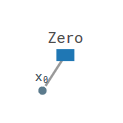
\includegraphics[]{./images/transformational_semantics_of_oz/var.png}}}%
\caption{variable as a channel}
\label{tra_var}%
\end{figure}


\section{Mapping operations}
\findex[process!operations]{}
\label{sec_tra_mapping_operation}
We map \oz{} class operations to \picalc{} channels as we did with state variables. That is, we map the operations $coffee, tea, talk$  of \refFig{oz_vm_reference_name} to \picalc{} channels $coffee, tea, talk$ as shown in \refFig{tra_var2}

\section{Mapping data Types}
\findex[process!data Types]{}
\label{sec_tra_mapping_data_types}
For simplicity, we do not implement any kind of type checking, but we deal with types by representing the value of the type by corresponding process. For example $cv: \{0,1,2,3\}$, means that the allowed processes to be initialized with $cv$ are: $Zero, One, Two, Three$.

\section{Mapping mathematical operators}
\findex[process!mathematical operators]{}
\label{sec_tra_mapping_mathematical_operations}
\subsubsection{\findex[process!addition]{Addition}:}
To add two numbers we use an addition process that mimics the behavior of arithmetic circuits for adding two bits binary numbers shown in 
\refFig{tra_adder_circuit}.
\refFig{tra_addition} shows visualization of the addition process and the ABC code.
The full implementation of $Add$ processes can be found in the appendix.
\begin{figure}[H]%
\centering
\fbox{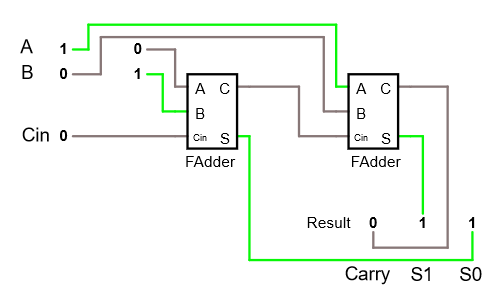
\includegraphics[keepaspectratio]{./images/transformational_semantics_of_oz/adder_circuit.png}}
\caption{adder circuit}
\label{tra_adder_circuit}%
\end{figure}


\begin{figure}[H]%
\centering
\subcaptionbox{ABC code.}{\fbox{$(\ \widehat{}\ \text{a,b,c}\ )\ (\ \text{Two}(\text{a})\ \mid\ \ \text{One}(\text{b})\ \mid\ \ \text{Add}(\text{a,b,c})\ )$}}%
\hspace{\fill}
\subcaptionbox{Before addition.}{\fbox{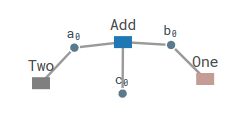
\includegraphics[keepaspectratio,width=0.45\textwidth]{./images/transformational_semantics_of_oz/add_before.png}}}%
\hspace{1em}%
\subcaptionbox{After addition.}{\fbox{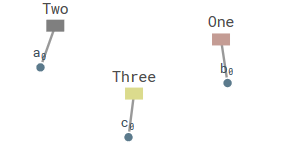
\includegraphics[keepaspectratio,width=0.45\textwidth]{./images/transformational_semantics_of_oz/add_after.png}}}%
\caption{addition as a process}
\label{tra_addition}%
\end{figure}


\subsubsection{\findex[process!subtraction]{Subtraction}:}
To subtract two numbers we use an subtraction process that mimics the behavior of arithmetic circuits for subtracting two bits binary numbers shown in 
\refFig{tra_subtract_circuit}.
\refFig{tra_subttraction} shows visualization of the subtraction process and the ABC code.
The full implementation of $Sub$ processes can be found in the appendix.
\begin{figure}[H]%
\centering
\fbox{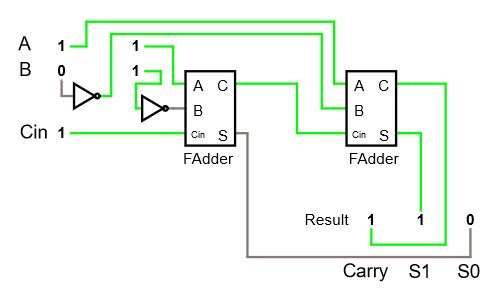
\includegraphics[keepaspectratio]{./images/transformational_semantics_of_oz/subtract_circuit.png}}
\caption{subtractor circuit}
\label{tra_subtract_circuit}%
\end{figure}
\begin{figure}[H]%
\centering
\subcaptionbox{Before subtraction.}{\fbox{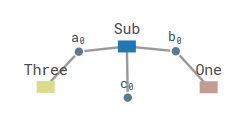
\includegraphics[keepaspectratio,width=0.45\textwidth]{./images/transformational_semantics_of_oz/sub_before.png}}}%
\hspace{1em}%
\subcaptionbox{After subtraction.}{\fbox{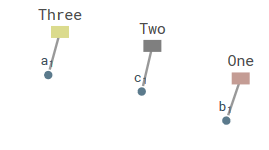
\includegraphics[keepaspectratio,width=0.45\textwidth]{./images/transformational_semantics_of_oz/sub_after.png}}}%
\vspace{2em}
\subcaptionbox{ABC code.}{\fbox{$(\ \widehat{}\ \text{a,b,c}\ )\ (\ \text{Three}(\text{a})\ \mid\ \ \text{One}(\text{b})\ \mid\ \ \text{Sub}(\text{a,b,c})\ )$}}%
\caption{subtraction as a process}
\label{tra_subttraction}%
\end{figure}


\subsubsection{\findex[process!comparation]{Comparation}}
To compare two numbers we need a processes that mimics the behavior of arithmetic circuits for comparing two bits binary numbers shown in 
\refFig{tra_comparator_circuit}.
\refFig{tra_comparation} shows visualization of the comparator process and the ABC code.
The full implementation of $Compare$ processes can be found in the appendix.
\begin{figure}[H]%
\centering
\fbox{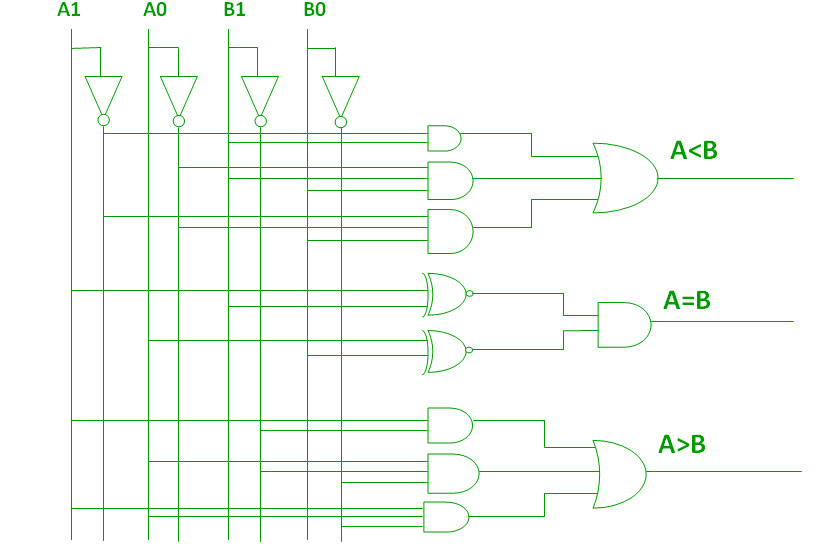
\includegraphics[keepaspectratio,width=0.85\textwidth]{./images/transformational_semantics_of_oz/comparator_circuit.png}}
\caption{comparator circuit}
\label{tra_comparator_circuit}%
\end{figure}


\begin{figure}[H]%
\centering
\subcaptionbox{Abc code.}{\fbox{$(\ \widehat{}\ \text{a,b,g,e,l}\ )\ (\ \text{Three}(\text{a})\ \mid\ \ \text{Two}(\text{b})\ \mid\ \ \text{Compare}(\text{a,b,g,e,l})\ \mid\ \ \text{Test}(\text{g,e,l})\ )$}}%
\hspace{\fill}
\subcaptionbox{Before comparation.}{\fbox{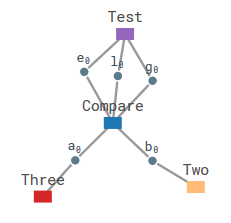
\includegraphics[keepaspectratio,width=0.45\textwidth]{./images/transformational_semantics_of_oz/comparator_before.png}}}%
\hspace{1em}%
\subcaptionbox{After comparation.}{\fbox{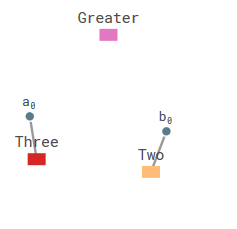
\includegraphics[keepaspectratio,width=0.45\textwidth]{./images/transformational_semantics_of_oz/comparator_after.png}}}%
\caption{comparation as a process}
\label{tra_comparation}%
\end{figure}


\subsubsection{\findex[process!set union and subtraction]{Set union and subtraction}:}
The implementation of set union and abstraction processes can be found in the appendix.



\section{Mapping OZ class}
\findex[process!OZ class]{}
\label{sec_tra_mapping_class}
\begin{figure}
\begin{subfigure}{.5\textwidth}
  \centering
\begin{class}{IdleShop(id: \integer)}
\begin{state}
m, vmId, self: \integer
\\t: nil | talk
\end{state} 
\\
\begin{init}
\\self = id
\\t = nil
\end{init} 
\\
\begin{op}{switch\_\_\_\_\ then\ ActiveShop}
\Delta (t)
\\x?: nil | talk
\ST
x? = t'
\end{op}
\end{class}
  \caption{1a}
  \label{fig:sfig1}
\end{subfigure}%
\begin{subfigure}{.5\textwidth}
  \centering
\fbox{  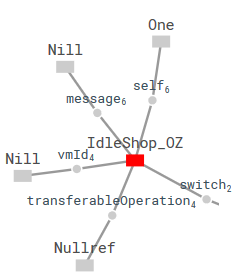
\includegraphics[width=.8\linewidth]{./images/transformational_semantics_of_oz/idleShop_OZ.png}}
  \caption{1b}
  \label{fig:sfig2}
\end{subfigure}
\vspace{2em}

\begin{subfigure}{1\textwidth}
  \centering
\lstinputlisting[backgroundcolor=\color{white},caption={ABC code: IdleShop OZ as a processes.},captionpos=b, label={idleShop_OZ}]{listings/idleShop_OZ.abc}
  \caption{1b}
  \label{fig:sfig3}
\end{subfigure}
\caption{transforming IdleShop}
\label{fig:fig}
\end{figure}

\section{Mapping transferable operation's variable}
\findex[process!transferable operation's variable]{}
\label{sec_tra_mapping_transferable_operation}
As mentioned in \refSec{sec_oz_dynamic_oz}, the mobility in Dynamic \oz{} is achieved
by attaching a distinguished variable transferableOperation for location. Location transferring
is mimicked by assigning a new location to that variable. To translate the variable transferableOperation into \picalc{} we cannot use \picalc{} channel as in \refSec{sec_tra_mapping_state_variables}, since the value of transferableOperation will be a channel name and not a processes representing a value like $Zero$. Thus, we map the variable transferableOperation to a channel named transferableOperation, where:

\begin{itemize}
\item transferableOperation = nil is mapped to Nullref(transferableOperation),

\item transferableOperation = talk is mapped to Ref(transferableOperation,talk),
\end{itemize}
as shown in \refFig{tra_ref} and \refLis{tra_ref_listing}.
\begin{figure}[H]%
\centering
\subcaptionbox{transferableOperation = nil.}{\fbox{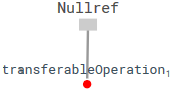
\includegraphics[keepaspectratio,width=0.45\textwidth]{./images/transformational_semantics_of_oz/transferableOperation_null.png}}}%
\hspace{\fill}
\hspace{1em}%
\subcaptionbox{transferableOperation = talk.}{\fbox{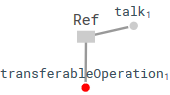
\includegraphics[keepaspectratio,width=0.45\textwidth]{./images/transformational_semantics_of_oz/transferableOperation.png}}}%
\caption{Mapping transferable operation's variable.}
\label{tra_ref}%
\end{figure}
\lstinputlisting[backgroundcolor=\color{white},caption={ Nullref and Ref processes in ABC code.},captionpos=b, label={tra_ref_listing}]{listings/ref_OZ.abc}
Thus using the concept of transferable operation's variable we can now transform the classes \textit{IdleShop} and \textit{ActiveShop} as shown in \refFig{tra_idleShop_OZ}, \refLis{tra_idleShop_OZ_listing} and \refFig{tra_activeShop_OZ}, \refLis{tra_activeShop_OZ_listing}.
\begin{figure}[H]
\begin{subfigure}{.6\textwidth}
\centering
\begin{class}{IdleShop(id: \integer)}
\\
\begin{state}
self, vmId, message: \integer
\\transferableOperation: nil | talk
\end{state} 
\\
\begin{init}
\\self = id
\\transferableOperation = nil
\end{init} 
\\
\begin{op}{switch\_\_\_\_\ then\ ActiveShop}
\Delta (transferableOperation)
\\x?: nil | talk
\ST
x? = transferableOperation'
\end{op}
\end{class}
  \caption{IdleShop class in OZ}
\end{subfigure}%
\begin{subfigure}{.4\textwidth}
  \centering
\fbox{  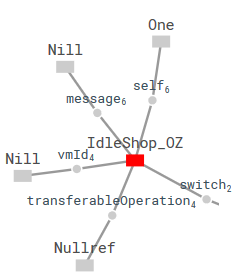
\includegraphics[width=.91\linewidth]{./images/transformational_semantics_of_oz/idleShop_OZ.png}}
  \caption{stargazer visualization}
\end{subfigure}
\caption{Transforming IdleShop into \picalc{} process IdleShop\_OZ\_PI}
\label{tra_idleShop_OZ}
\end{figure}

\lstinputlisting[backgroundcolor=\color{white},caption={The process IdleShop\_OZ\_PI in ABC code.},captionpos=b, label={tra_idleShop_OZ_listing}]{listings/idleShop_OZ.abc}
\begin{figure}[H]
\begin{subfigure}{.6\textwidth}
\centering
\begin{class}{ActiveShop(id: \integer)}
\\
\begin{state}
self, vmId, message: \integer
\\transferableOperation: nil | talk
\end{state} 
\\
\begin{init}
\\self = id
\\transferableOperation = talk
\end{init} 
\\
\begin{op}{switch\_\_\_\_\ then\ IdleShop}
x!: nil | talk
\ST
x! = transferableOperation
\\transferableOperation' = nil
\end{op}
\\
\begin{op}{talk}
\Delta (vmId, message)
\\y?, z?: \integer
\ST
y? = message'
\\z? = vmId'
\end{op}
\end{class}
  \caption{ActiveShop OZ class}
\end{subfigure}%
\begin{subfigure}{.4\textwidth}
  \centering
\fbox{  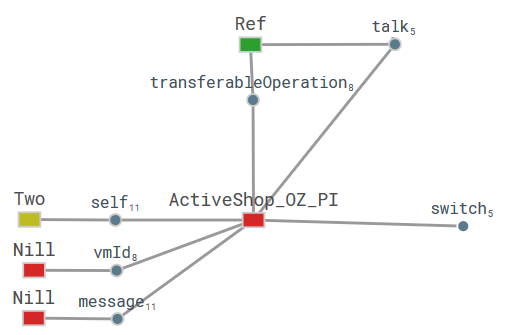
\includegraphics[width=.91\linewidth]{./images/transformational_semantics_of_oz/activeShop_OZ.png}}
  \caption{stargazer visualization}
\end{subfigure}
\caption{transforming ActiveShop into \picalc{} process ActiveShop\_OZ}
\label{tra_activeShop_OZ}
\end{figure}

\lstinputlisting[backgroundcolor=\color{white},caption={ ActiveShop OZ class as a process in ABC code.},captionpos=b, label={tra_activeShop_OZ_listing}]{listings/activeShop_OZ.abc}

Finally, \refFig{tra_system_before}, \refFig{tra_system_after} and \refLis{tra_system_lis} show the big picture of a system consisting of two shops, a vending machine and a customer. The full implementation can be found in the appendix.
\begin{figure}[H]%
\centering
\subcaptionbox{Before switching.}{\fbox{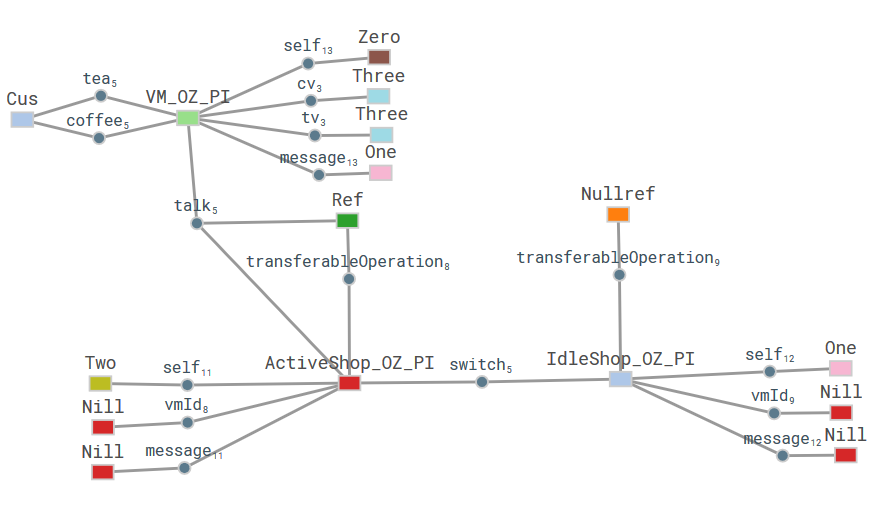
\includegraphics[keepaspectratio,width=0.45\textwidth]{./images/transformational_semantics_of_oz/all_switch_before.png}}}%
\hspace{1em}%
\subcaptionbox{After switching.}{\fbox{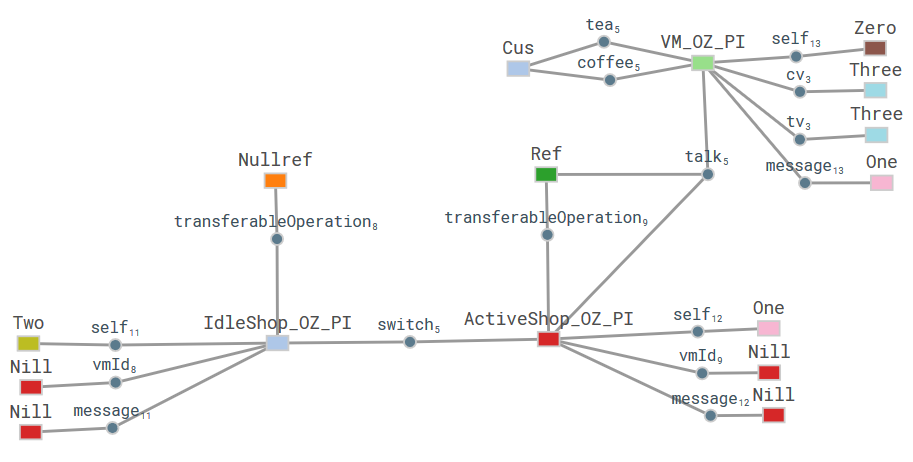
\includegraphics[keepaspectratio,width=0.45\textwidth]{./images/transformational_semantics_of_oz/all_after_switch.png}}}%
\caption{comparation as a process}
\label{tra_system}%
\end{figure}

\lstinputlisting[backgroundcolor=\color{white},caption={ system consisting of: two shops, vending machine and a customer.},captionpos=b, label={tra_system_lis}]{listings/system.abc}

